\section{Definitions}
\label{sec:definitions}

\cbstart
One of reasons to present an ontology is to enable sharing of knowledge between people. Therefore, it is important that the terms we use are clearly defined. When presenting our ontology in \cref{sec:ontology}, we will formalize the terms such that it can be used by software agents, but first we will define the terms linguistically, such that communication among different people is clear when these people conform to our ontology. We will first define the concept of a scenario. Next, we will define two important attributes of a scenario, events and activities, in \cref{sec:event,sec:activity}, respectively. Lastly, we will present the definition of a scenario class in \cref{sec:scenario class}.
\cbend



\subsection{Scenario}
\label{sec:scenario}

% Definition according to Go and Carroll
\textcite{go2004blind} describe a scenario within the field of system design. They define a scenario as ``a description that contains (1) actors, (2) background information on the actors and assumptions about their environment, (3) actors' goals or objectives, and (4) sequences of actions and events. Some applications may omit one of the elements or they may simply or implicitly express it. Although, in general, the elements of scenarios are the same in any field, the use of scenarios is quite different.'' 

% Definition according to Geyer et al.
\textcite{geyer2014} describe a scenario within the context of automated driving. They use the metaphor of a movie or a storybook for describing a scenario. \textcite{geyer2014} state that ``a scenario includes at least one situation within a scene including the scenery and dynamic elements. However, [a] scenario further includes the ongoing activity of one or both actors.'' For a further explanation of the terms situation, scene, and scenery, see \cite{geyer2014}. It is mentioned that the action of the driver and/or automation might be predefined. In \cite{geyer2014}, the meaning of action is not detailed.
%In an example of a so-called crossway scenario, they mention that the course of events might be different. For example, when a car keeps constant speed and then turns right, the scenario consists of one situation. The car might also first decelerate, accelerate and decelerate before turning right. In this case, the scenario consists of four situations.

% Definition according to Ulbrich et al.
\textcite{ulbrich2015} also define a scenario in the context of automated driving. They define a scenario as ``the temporal development between several scenes in a sequence of scenes. Every scenario starts with an initial scene. Actions \& events as well as goals \& values may be specified to characterize this temporal development in a scenario. Other than a scene, a scenario spans a certain amount of time.'' They state that actions and events link the different scenes. A further description of actions and events is not given in \cite{ulbrich2015}.

% Definition according to Elrofai et al.
Another definition of a scenario in the context of automated driving is given by \textcite{elrofai2016scenario}. They define scenario as ``the combination of actions and maneuvers of the host vehicle in the passive [i.e., static] environment, and the ongoing activities and maneuvers of the immediate surrounding active [i.e., dynamic] environment for a certain period of time.'' They further mention that the duration of a scenario typically is in the order of seconds.

% "Requirements"
Before providing the definition of the notion of scenario, the characteristics of this notion are listed.

% Order of seconds
\subsubsection{A scenario corresponds to a time interval}
The aforementioned definitions \cite{go2004blind, geyer2014, ulbrich2015, elrofai2016scenario} state that a scenario corresponds to a time interval. \textcite{vannotten2003updated} call such a scenario a chain scenario (``like movies''), as opposed to a snapshot scenario, i.e., a scenario that describes the state at a time instant (``like photos''). The duration of a scenario is in the order of seconds, as explicitly mentioned by \textcite{elrofai2016scenario}. Though the duration is not mentioned by \textcite{ulbrich2015}, the presented example is in the order of seconds. Furthermore, other scenarios regarding (automated) driving are also in the order of seconds, e.g., see \cite{gietelink2006development, zofka2015datadrivetrafficscenarios, roesener2017comprehensive, karaduman2013interactivebehavior, hulshof2013autonomous, englund2016grand}.

% Scenarios consists of one or several events
\subsubsection{A scenario consists of one or several events \cite{vannotten2003updated, go2004blind, geyer2014, ulbrich2015, kahn1962, englund2016grand, schoemaker1993multiple, cuppens2002alert, bach2016modelbased}}
It can be helpful to develop scenarios using events \cite{bishop2007scentechniques}. Thus, a scenario could be defined as a particular sequence of events or, as \textcite{kahn1962} writes, ``a scenario results from an attempt to describe in more or less detail some hypothetical sequence of events''. Furthermore, \textcite{geyer2014} and \textcite{ulbrich2015} use the notion of event for describing a scenario, although they do not provide a definition of the term \emph{event}. In \cref{sec:event}, we will elaborate on the notion of \emph{event}.

% Semantically described
\subsubsection{Real-world traffic scenarios are quantitative scenarios}
Regarding the nature of the data, a scenario can be either qualitative or quantitative \cite{vannotten2003updated}. Real-world traffic scenarios are quantitative scenarios, such that they are, e.g., suitable for simulation purposes. A scenario, however, can be described qualitatively, such that it is readable and understandable for human experts. Providing a qualitative description of a quantitative scenario has become known as a story-and-simulation approach \cite{alcamo2001scenarios}. Note that several quantitative scenarios might have the same qualitative description; thus a qualitative description of a scenario does not uniquely define a quantitative scenario. A qualitative description can be regarded as an abstraction of the quantitative scenario.

% Some relevance between events
\subsubsection{The time interval of a scenario contains all relevant events}
According to \textcite{geyer2014}, ``the end of a scenario is defined by the first irrelevant situation with respect to the scenario''. In a similar manner, we require that the time interval of a scenario should contain all relevant events. Note that `relevant' is subjective and, therefore, an event is considered to be relevant, if it is relevant to the ego vehicle.
% Next to that, an event is regarded as irrelevant, if it is independent of the relevant events.

% Goals (instead of activities)
\subsubsection{A scenario can contain goal(s) of one or multiple actors}
For describing a scenario in real-world data, it is not necessary to describe the goals and therefore, \textcite{elrofai2016scenario} do not mention this. When describing a scenario that an AV has to cope with, however, its goals (i.e., its driving mission \cite{geyer2014}) could be specified rather than its activities \cite{ulbrich2015}. The same holds for other actors within the scenario.

% Description of static environment
\subsubsection{A scenario includes the description of the environment}
A scenario should include the description of the static and dynamic environment. The static environment does not change during a scenario. Although this is not a general prerequisite of a scenario, the description of the static environment is often included when speaking about traffic scenarios \cite{geyer2014, ulbrich2015, elrofai2016scenario, ebner2011identifying, schuldt2013effiziente, althoff2017CommonRoad}. Everything that changes during the time interval of a scenario is considered to be part of the dynamic environment. 

% Definition
Hence, we define a scenario as follows.
\begin{definition}[Scenario]\label{def:scenario}
	A scenario is a quantitative description of the ego vehicle, its activities and/or goals, its static environment, and its dynamic environment. From the perspective of the ego vehicle, a scenario contains all relevant events.
\end{definition}

% Describe difference from literature
% - quantitative --> to avoid ambiguous situation and to serve assessment
% - notion of scene not used. Scene follows from description, but is not explicitely used
\Cref{def:scenario} deviates from existing definitions \cite{geyer2014, ulbrich2015, elrofai2016scenario} in that it explicitly mentions that a scenario is quantitative. We use the term \emph{scenario class} to refer to the qualitative description, see \cref{sec:scenario class}.

\textcite{geyer2014} and \textcite{ulbrich2015} use the term \emph{scene} to define a scenario, while \cref{def:scenario} describes the scenes implicitly. Thus the scenes do not have to be described explicitly.

\Cref{fig:scenario} provides a schematic overview of the various components of a scenario. As shown in the second row of \cref{fig:scenario}, a scenario contains a description of the ego vehicle, the dynamic environment, and the static environment. As an example, possible activities of the vehicle in front, which is part of the dynamic environment, are detailed by considering the states `heading' and `speed'. \cbstart Note that a definition of the term activity is given in \cref{sec:activity}\cbend. The two rows of the activities show more generic descriptions and more detailed descriptions, respectively, of some possible activities.

\begin{figure}
	\centering
	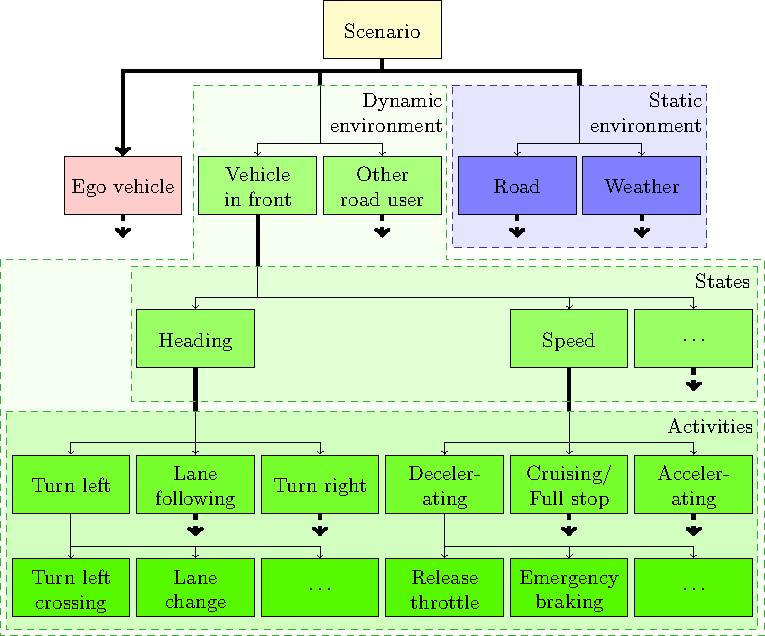
\includegraphics[width=\linewidth]{figures/scenario.pdf}%
	\caption{Schematic overview of a scenario. Note that the dynamic environment is not limited to the `vehicle in front' and `other road user', while the static environment is not limited to `road' and `weather'.}
	\label{fig:scenario}
\end{figure}



\subsection{Event}
\label{sec:event}
% Introduction of this section
As mentioned earlier, a scenario consists of events. Events can be seen as the building blocks of a scenario. The notion of event is extensively used in literature \cite{breu1997towards, kim1993supervenience, pfeiffer2013concepts, branicky1998hybridcontrol, deschutter2000optimal, heemels2012eventcontrol}. In this section, a selected number of descriptions is presented. Next, a definition of event is given that suits our context.

% Literature review
The term event is used in many different fields, e.g.:
\begin{itemize}
	\item In computing \cite{breu1997towards}, an event is an action or occurrence recognized by software. A common source of events are inputs by the software users. An event may trigger a state transition.
	\item \textcite{kim1993supervenience}, a philosopher, writes: ``The term event ordinarily implies change''. \textcite{kim1993supervenience} states that an event is composed of three elements: objects, a property, and a time instant or a temporal interval. 
	\item In probability theory, an event is an outcome or a set of outcomes of an experiment \cite{pfeiffer2013concepts}. For example, a thrown coin landing on its tail is an event.
	%\item ``In relativity, an event is any occurrence with which a definite time and a definite location are associated; it is an idealization in the sense that any actual event is bound to have a finite extent both in time and in space'' \cite{sartori1996understanding}.
	\item In the field of hybrid theory, ``the continuous and discrete dynamics interact at `event' or `trigger' times when the continuous state hits certain prescribed sets in the continuous state space'' \cite{branicky1998hybridcontrol}. ``A hybrid system can be in one of several modes, [...], and the system switches from one mode to another due to the occurrence of events'' \cite{deschutter2000optimal}.
	\item In event-based control, a control action is computed when an event is triggered, as opposed to the more traditional approach where a control action is periodically computed \cite{heemels2012eventcontrol}. 
\end{itemize}

Before providing the definition of an event, the following is concluded about an event:

% It is a time instant
\subsubsection{An event corresponds to a time instant}
Whether it is regarding computing, hybrid control, or event-based control, an event is happening at a time instant.

% Event should mark transition of a state from one set to another - mention relation with hybrid control
\subsubsection{An event marks a mode transition}
A mode transition may be caused by either an abrupt change of an input signal, a change of a parameter or a change in the model. For example, pushing the brake pedal may cause a mode transition and therefore, this may be regarded as an event. 

%\subsubsection{An event marks (a cause of) a mode transition}
%Events mark the transition of mode, which is either a change of input, parameter or state. This is analogous to the way event is described in hybrid control \cite{boel1999hybridcontrol}.

% Give definition
Hence, we define an event as follows.
\begin{definition}[Event] \label{def:event}
	An event marks the time instant at which a mode transition occurs, such that before and after an event, the state corresponds to two different modes.
\end{definition}

% Compare definition with literature and other remarks
% - Mention that it is basically similar to the definition adopted with hybrid control theory
% - Mention that before and after, different qualitative description
An event according to \cref{def:event} is related to an event described in hybrid control \cite{deschutter2000optimal}, where an event describes the transition from one mode of operation to another mode of operation. In our application, i.e., events in traffic scenarios, ``mode of operation'' is described by a certain model with parameters assigned to it.

%The inter-event time interval, i.e., the time in between two events, corresponds to a certain activity. For example, when the longitudinal acceleration is negative during an inter-event time interval, the activity can be described by the label `braking'.
%Another example of an event is the time instant at which the head lights are turned on. In that case, the activities before and after the event can be described as `lights off' and `lights on', respectively.


\cbstart
\subsection{Activity}
\label{sec:activity}

As mentioned in \cref{sec:dynamic environment}, the dynamic environment consists of the moving actors. To describe the dynamic environment, activities are used. The activities describe the way the states evolve over time. 

An activity refers to the behavior of a particular mode. For example, an activity could be described by the label `braking' or `changing lane'.
A scenario contains the quantitative description of the ongoing activity of the ego vehicle and its dynamic environment. Here, the description refers to the changing states that are relevant for the scenario, e.g., acceleration and velocity. The activity is described using the models that describe the way the state evolves over time.

\color{red}
TODO:
\begin{itemize}
	\item Give definition of activity and a bit more explanation.
	\item Explain difference between action and activity (which also explains why we do not use the term action).
\end{itemize}
\color{black}

\cbend

\subsection{Scenario class}
\label{sec:scenario class}

% Introduce term scenario class (i.e. qualitative description of scenario)
In this section, the notion of scenario class is introduced. As proposed above, a scenario in the context of the performance assessment of an AV needs to be quantitative. However, a qualitative description of each scenario exists. 
A scenario class refers to the qualitative description of a scenario.
The qualitative description can be regarded as an abstraction of the quantitative scenario. Therefore, a scenario class refers to multiple scenarios with a common characteristic \cite{elrofai2018scenario}.
\cbstart
We define a scenario class as follows.
\begin{definition}[Scenario class] \label{def:scenario class}
	A scenario class refers to a set of scenarios that are qualitatively described similarly.
\end{definition}
\cbend

% What is the purpose of this?
% - Human interpretable
% - Group scenarios that are very similar --> Analysis is easier
% - Completeness

Introducing the concept of scenario classes brings the following benefits:
\begin{itemize}
	\item Whereas the quantitative description might be difficult to interpret as a human, a qualitative description is more easily interpreted by a human.
	\item It enables to refer to a group of scenarios that have something in common. This makes communication much easier.
	\item It enables easier comparison of scenarios. This can be used to quantify the completeness of a set of scenarios; see \cite{degelder2019completeness} for more details on this.
\end{itemize}

% Explain scenarios fall into scenario class
\cbstart
We describe the formal relation between a scenario and a scenario class with the verb ``to fall into'', denoted by $\in$. If a specific scenario class $\mathcal{C}$ is an abstraction of a specific scenario $S$, then we say that the specific scenario $S$ falls into that specific scenario class $\mathcal{C}$, or simply $S \in \mathcal{C}$\cbend. Multiple scenarios can fall into a given scenario class. For example, consider the scenario class with the name ``Day'', see \cref{fig:venn diagram scenario class}. All scenarios that occur during the day fall into the scenario class ``Day''.

\setlength{\venncircle}{7em}
\begin{figure}
	\centering
	\begin{tikzpicture}
	\fill[red, fill opacity=0.5] (-\venncircle/2, 0) circle (\venncircle);
	\fill[green, fill opacity=0.5] (\venncircle/2, 0) circle (\venncircle);
	\draw (-\venncircle/2, 0) circle (\venncircle);
	\draw (\venncircle/2, 0) circle (\venncircle);
	
	\node[anchor=east](daylight) at (-4/3*\venncircle, 3/4*\venncircle) {Day};
	\draw (daylight) -- ({(-sqrt(3)/2-1/2)*\venncircle}, \venncircle/2);
	\node[anchor=west](rain) at (4/3*\venncircle, 3/4*\venncircle) {Rain};
	\draw (rain) -- ({(sqrt(3)/2+1/2)*\venncircle}, \venncircle/2);
	
	\node[text width=\venncircle, align=center] at (-\venncircle, 0) {Scenarios without rain during day};
	\node[text width=\venncircle, align=center] at (0, 0) {Scenarios with rain during day};
	\node[text width=.9\venncircle, align=center] at (\venncircle, 0) {Scenarios with rain during night};
	\end{tikzpicture}
	\caption{The red and green circles correspond to the scenario classes ``Day'' and ``Rain'', respectively. Scenarios that occur during the day with rain fall into both scenario classes ``Day'' and ``Rain''. The new scenario class ``Day and rain'' can be defined as the scenario class in which all scenarios that occur during the day with rain fall. The scenario class ``Day and rain'' falls into the scenario classes ``Day'' and ``Rain''.}
	\label{fig:venn diagram scenario class}
\end{figure}

% Explain scenario can fall into multiple scenario classes
Whereas multiple scenarios can fall into one scenario class, it is also possible for one scenario to fall into multiple scenario classes. Continuing the example of \cref{fig:venn diagram scenario class}, a scenario with rain during the day falls into both the scenario classes ``Day'' and ``Rain''.

% Explain scenario class can fall into scenario classes
\cbstart
The verb ``to fall into'' is also used to describe the relation between two scenario classes. A scenario class $\mathcal{C}_1$ is said to fall into a scenario class $\mathcal{C}_2$ if all scenarios that fall into scenario class $\mathcal{C}_1$ also fall into scenario class $\mathcal{C}_2$. In that case, we can write $\mathcal{C}_1 \subseteq \mathcal{C}_2$. Thus we have
\begin{equation}
	\mathcal{C}_1 \subseteq \mathcal{C}_2 \text{ if } S \in \mathcal{C}_2 \,\,\forall\,\, S \in \mathcal{C}_1.
\end{equation}
\cbend
For example, consider the scenario class ``Rain during day'', which is represented by the intersection of the red and green circles in \cref{fig:venn diagram scenario class}. All scenarios with rain that occur during the day fall into this scenario class. Obviously, these scenarios also fall into the scenario classes ``Day'' and ``Rain''. Hence, the scenario class ``Rain during day'' falls into the scenario classes ``Day'' and ``Rain''.

When providing extra information to a piece of data, often tags are used \cite{smith2007tagging}. A tag is a keyword or a term that helps describing an item. For example, items in a database can contain some tags that enable users to quickly obtain several items that share a certain characteristic described by a tag \cite{craft2004tagging, vasquez2019controlling}. Applications are very broad, e.g., from classification of audio data \cite{kong2017joint} and capturing musical characteristics from songs \cite{ellis2011semantic} to tagging of Wikipedia pages \cite{voss2006collaborative}.

It is proposed to provide scenarios and scenario classes with tags that describe the scenario in a qualitative manner. The tags of a scenario determines which scenario classes the scenario falls into. For example, if a scenario occurred during the day, it will contain the tag ``Day''. As a result, the scenario is automatically recognized as a scenario that falls into the scenario class ``Day'' which is characterized by the single tag ``Day''. The use of these tags brings some benefits:
\begin{itemize}
	\item The scenarios do not need to be directly classified. This can be a time-consuming effort if the number of scenario classes is high.
	\item If a scenario class that only contains known tags is added to the database of scenario classes, it can be easily seen which scenarios fall into this scenario class by only inspecting the tags of the scenarios.
	\item It is easy to select scenarios from a scenario database or a scenario library by using tags or a combination of tags.
\end{itemize}

There is a balance between having generic scenario classes - and thus a high variety among the scenarios belonging to the scenario class - and having specific scenario classes without much variety among the scenarios in the scenario class. For some systems, one may be interested in very specific set of scenarios, while for another system one might be interested in a set of scenarios with a high variety. To accommodate this, tags are structured in hierarchical trees \cite{molloy2017dynamic, badger2012dynamic}. The different layers of the trees can be regarded as different abstraction levels \cite{Bonnin2014}. 

In \cite{degelder2019scenarioclasses}, several trees of tags are defined and \cref{fig:tree vehicle activities} shows two examples of trees of tags taken from \cite{degelder2019scenarioclasses}. These tags describe possible activities of a vehicle, i.e., the lateral motion control (via steering) and longitudinal motion control (via acceleration and deceleration) are reflected into tags. The tags may refer to the objective of the ego vehicle in case no activities are defined. For example, a test case in which the ego vehicle's objective is to make a left turn, the tags ``Turning'' and ``Left'' are applicable. 

\begin{figure*}
	\centering
	\begin{subfigure}{\linewidth}
		\centering
		\tree{Vehicle lateral activity}{Going straight; Changing lane, Left, Right; Turning, Left, Right; Swerving, Left, Right}
		\caption{Lateral activities of a vehicle.}
		\label{fig:tree vehicle lat act}
	\end{subfigure}
	\begin{subfigure}{\linewidth}
		\centering
		\tree{Vehicle longitudinal activity}{Reversing; Standing still; Driving forward, Braking, Cruising, Accelerating}
		\caption{Longitudinal activities of a vehicle.}
		\label{fig:tree vehicle long act}
	\end{subfigure}
	\caption{Tags for lateral and longitudinal activities of a vehicle. The lateral activity is relative to the lane in which the corresponding vehicle is driving. For example, if the vehicle is driving on a curved road, its lateral activity is ``Going straight''.}
	\label{fig:tree vehicle activities}
\end{figure*}

Four different types of activities are identified regarding the lateral movement, see \cref{fig:tree vehicle lat act}. Here, it is assumed that ``Lateral'' refers to the direction perpendicular to the lane the vehicle is driving in (e.g., according to the Road Coordinate System in \cite{zofka2015datadrivetrafficscenarios}). Therefore, if the vehicle is driving on a curved road while staying more or less in its lane (lane-following), the tag ``Going straight'' is applicable. \cbstart Besides going straight, the vehicle might change lane, turn, or swerve to either the left or the right.\cbend

